% Review Christian Stary January 2020

%appendix in smaller font size
\footnotesize

\captionsetup{font=footnotesize}
\setminted{fontsize=\footnotesize}
\setmintedinline{fontsize=\footnotesize,breaklines}

The CoreASM PASS Reference Implementation is based on theoretical works
by Egon Börger~\cite{boerger2011interpreter} and Manuel Bandmann~\cite{bandmann2014spezifikation}, which predate
the OWL description, and incorporates concepts, that are not (yet) part of the agreed PASS Standard and OWL description.
The first goal of the reference implementation was to enable the interactive process model validation
based on formal PASS execution semantics, i.e. to demonstrate that the specification is actually executable and sound.
In order to reach that goal not all known PASS concepts could be implemented at once, for example
only one InputPoolConstraintStrategy is currently implemented.
Section~\ref{CoreASM-Reference-Implementation-Differences-OWL-Model} describes the conceptual differences and
missing elements to the OWL description.

The bigger part of this appendix lists relevant Abstract State Machines (ASM)~\cite{book:ASM-2003} rules
in the CoreASM dialect in an edited form,
see section~\ref{CoreASM-Reference-Implementation-Editorial-Note} for the applied editorial changes.

The full CoreASM PASS Reference Implementation is publicly available at~\cite{Web:PASS-CoreASM}.
The following section~\ref{CoreASM-Reference-Implementation-Architecture} gives an overview of the
main elements of the reference implementation.


\section{Architecture}
\label{CoreASM-Reference-Implementation-Architecture}

\begin{figure}[htbp]
    \centering
    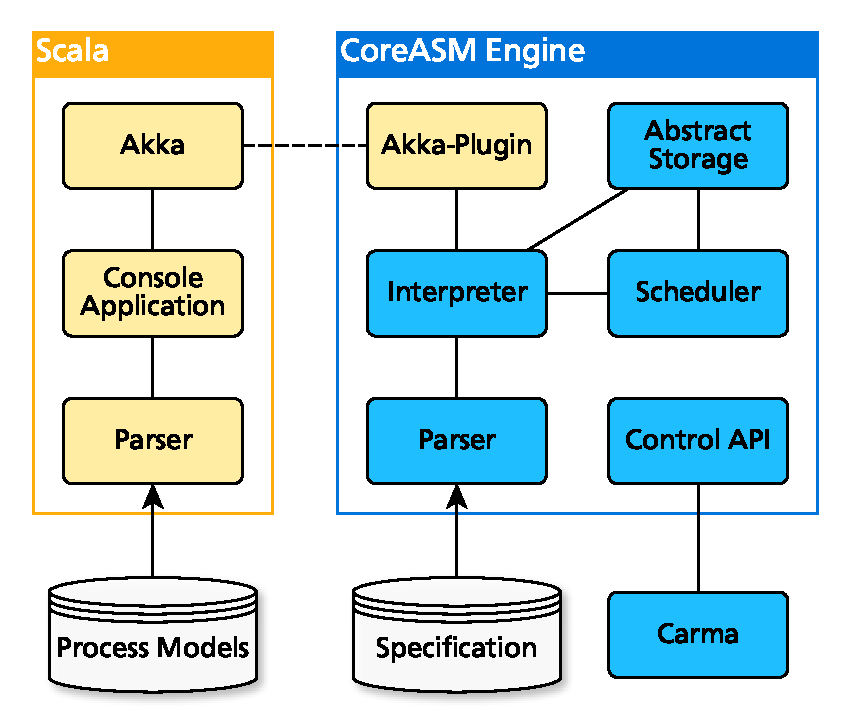
\includegraphics[width=0.7\linewidth]{Figures/CoreASM/ArchitekturKonsoleCoreASM}
    \caption{Architecture of the reference implementation}
    \label{fig:coreasm_architecture}
\end{figure}

% Runtime environments and system components.
% The blue (dark background) components are existing parts of the Java based CoreASM Engine.
% The yellow (light background) components are developed for the PASS-interpreter.

The overall architecture of the CoreASM PASS Reference Implementation is shown in
figure~\ref{fig:coreasm_architecture} and consists on the top level of
a console application as user interface and the CoreASM Engine as execution environment for the PASS-interpreter specification.
For stability and performance improvements the fork~\cite{Web:CoreASM-Fork} of the CoreASM framework~\cite{Farahbod2011} is used.
Both high level components are running in parallel in separate Java Virtual Machine processes.
The PASS-interpreter specification file includes an ASM specification of asynchronous multi-agent ASMs,
executing each Subject instance by one ASM-agent each.


The CoreASM Engine parses the specification file and executes the rules in the interpreter
in cooperation with the abstract storage and the scheduler.
The abstract storage stores the state of the ASM and is also used to support
TurboASMs and their submachine states.

The scheduler is used to support asynchronous multi-agent ASMs; with
the \textit{default} scheduling policy it selects
a random subset of the running ASM agents and calls the
interpreter for the parallel evaluation of their main rules.
If the resultant update sets
are consistent they are applied in the abstract storage, otherwise the scheduler
selects a different subset of the running ASM agents for a re-evaluation.
Supplementary the \textit{onebyone} scheduling policy can be used to evaluate
only a single agent per step and the \textit{allfirst} policy can be used
to attempt to evaluate all agents at once before falling back
to the default scheduling policy in case of inconsistencies.
The reference implementation uses the \textit{allfirst} scheduling policy for performance reasons,
but the \textit{default} policy could be used as well.

The Carma application is a simple Java application provided by the CoreASM framework
to allow the usage of the CoreASM engine as standalone application in a command line.

The console application is developed in Scala.
A user can load, start and execute locally stored PASS process model files with it.
The interaction between the console application and the CoreASM engine is realized by Akka actors.
The Akka actor of the engine has full read and write access to all CoreASM functions by using a Plug-In interface.



\section{Conceptual Differences to the OWL Description}
\label{CoreASM-Reference-Implementation-Differences-OWL-Model}

\definecolor{OWLClass}{RGB}{207, 165, 0}
\definecolor{OWLObjectProperty}{RGB}{0, 121, 186}
\definecolor{OWLDataProperty}{RGB}{56, 161, 74}
\definecolor{OWLIndividual}{RGB}{135, 75, 130}

\newcommand\OWLClass[1]{{\textcolor{OWLClass}{\textbf{#1}}}}
\newcommand\OWLObjectProperty[1]{{\textcolor{OWLObjectProperty}{\textbf{#1}}}}
\newcommand\OWLDataProperty[1]{{\textcolor{OWLDataProperty}{\textbf{#1}}}}
\newcommand\OWLIndividual[1]{{\textcolor{OWLIndividual}{\textbf{#1}}}}


% NOTE: Some content might move to Appendix B / replace it.
% TODO: Introduce history (Börger -> Bandmann -> Wolski)? Explain focus on Interaction Soundness or remove it?

% functions span over a state function and transition function.
% the state function determines which transitions are enabled and prepares the transition action.
% example receive function: state function checks IP, transition function removes message from it and stores it in a variable.


%This reference implementation has some conceptual differences to the OWL description.
%\comment[id=CS]{is there an overall rationale for that?}
%\comment[id=AW]{historical reasons - it was created before the OWL description and is since converging. Also based on concepts of the S-BPM Groupware, which has advanced features, that are not part of the OWL description.}

%For example it provides less flexible InputPool constraints and does not support synchronous communication,
%however it supports advanced features that are required for distributed inter-company business processes
%and provides concrete implementations for the usage of Subject Data.

\begin{table}[htbp]
    \footnotesize
	\centering
    \begin{tabular}[t]{@{}p{0.23\linewidth} p{0.35\linewidth} p{0.35\linewidth} @{}}
        \toprule
        Concept & Reference Implementation & Corresponding OWL Element Description \\
        \midrule

        % included in Chapter 3
        InputPool
        &
        Exactly one limit has to be defined for each Subject, the value 0 means the InputPool is not limited.
        The limit applies to each pair of (Sender, MessageType).
        Only \OWLIndividual{InputPoolConstraintStrategy-Blocking} is supported, synchronous send \& receive is not supported.
        &
        Allows exact limits for different Subjects and MessageTypes.
        The combination \OWLIndividual{InputPoolConstraintStrategy-Blocking} with the limit of 0 means synchronous send \& receive.
        Additionally defines the strategies DeleteLatest, DeleteOldest and Drop.
        \\

        % included in Chapter 3
        Subject Restart
        &
        Automatically when an additional message arrives on a Subject that is \textit{proper terminated}.
        &
        \textit{Absent}.
        \\

        % included in Chapter 3
        Proper Termination
        &
        When a Subject terminates and its InputPool is empty it is \textit{proper terminated} and can be restarted.
        %On termination of a Subject it determines if the InputPool is empty and a Subject Restart is allowed.
        %If the InputPool is not empty further messages are blocked and the Subject is not allowed to restart.
        &
        \textit{Absent}.
        \\

        % included in Chapter 3
        End State
        &
        Continuing the Subject behavior is not supported.
        Implemented as \OWLClass{TerminateFunction}, which determines \textit{proper termination} and enables \textit{subject restart}.
        It must not have any outgoing transitions.
        &
        An \OWLClass{EndState} on a \OWLClass{DoState} or \OWLClass{ReceiveState} with an outgoing transition allows to continue the Subject behavior.
        \\

        % included in Chapter 3
        Choice Segments
        &
        A Choice Segment begins with a Modal Split state. The paths are joined in a Modal Join state.
        The target State of every outgoing Transition from the Modal Split State is an \OWLClass{InitialStateOfChoiceSegmentPath}.
        Every Choice Segment Path is mandatory to start and mandatory to end.
        &
        A Choice Segment is a single State.
        Choice Segment Paths can be both optional to start and optional to end.
        Choice Segment Paths are not connected by Transitions to the \OWLClass{ChoiceSegment} state. % or its target State.
        \\

        \bottomrule
    \end{tabular}
    \caption{Key Conceptual Differences}
    \label{tbl:asm:concepts_1}
\end{table}

The most important differences are listed in Table~\ref{tbl:asm:concepts_1}:
while the corresponding OWL Element Description offers both synchronous and asynchronous communication, different InputPool limits and handling strategies
this reference implementation addresses only asynchronous communication with a blocking strategy.
The End State property is not supported, but instead a Terminate Function is used.
%Conceptually the End State is not a property of a state, but provides a distinguished function specification
%to terminate a Subject and determine the \textit{proper termination}, which is required for the verification on interaction soundness.
Next, the execution of Choice Segment Paths is not controlled by a Choice Segment State, but those paths have to be started with a Modal Split Function and joined in a Modal Join Function.

\begin{table}[htbp]
    \footnotesize
	\centering
    \begin{tabular}[t]{@{}p{0.23\linewidth} p{0.35\linewidth} p{0.35\linewidth} @{}}
        \toprule
        Concept & Reference Implementation & Corresponding OWL Element Description \\
        \midrule

        % included in Chapter 3
        CorrelationID
        &
        Concept to correlate messages, e.g. responses to requests, so that messages can be send and received reliable in a loop.
        &
        \textit{Absent}.
        \\

        % included in Chapter 3
        InputPool Functions
        &
        InputPool Functions perform operations on the Subject's InputPool, e.g. close it for some message types or sender Subjects.
        &
        \textit{Absent}.
        \\

        % not shown in Chapter 3
        Timer Transition
        &
        The Timer Transition Condition has to be defined in seconds.
        &
        It is possible to define the timeout in arbitrary time durations, including in business days.
        \\

        % not shown in Chapter 3
        Reminder Transition
        &
        \textit{Absent}.
        &
        A \OWLClass{ReminderTransition} can be traversed if a certain time based event or frequency has been reached.
        \\

        % included in Chapter 3
        Mobility of Channels
        &
        Concept to store and forward at runtime references to other subjects and their agents.
        &
        \textit{Absent}.
        \\

        % included in Chapter 3
        Macro Exit Parameter
        &
        Attribute on the End State of a Macro Behavior that selects a corresponding Transition on the \OWLClass{MacroState}.
        &
        \textit{Absent}
        \\

        Maximum Subject \par Instances
        &
        \textit{Absent}. Every Subject can have an arbitrary amount of instances.
        &
        The \OWLDataProperty{hasMaximumSubjectInstanceRestriction} property limits the amount of instances that can be created at runtime of a Subject.
        \\

        \bottomrule
    \end{tabular}
    \caption{Further Conceptual Differences}
    \label{tbl:asm:concepts_2}
\end{table}

In Table~\ref{tbl:asm:concepts_2} further important conceptual differences are listed:
CorrelationIDs define a relation between messages and allow reliable looped communication patterns.
CorrelationIDs appear as metadata of a message and as argument to an InputPool queue:
A CorrelationID is created when a message is send and part of it. A later message, that relates to it, will be send to the InputPool queue of that CorrelationID,
allowing a receive state to specify that only specific messages can be received.
With the InputPool Functions queues of the InputPool can be opened and closed, forcing senders to block if they attempt to send to a closed queue.
Also, the InputPool can be checked if it is empty or not, so that \textit{non-proper termination} can be avoided.
As this reference implementation targets an interactive process model validation only timeouts in seconds are considered.
With the Mobility of Channels concept it is possible to store runtime references to agents as Subject Data and to communicate those references with other Subjects,
which enables various distributed communication patterns.
Macro Exit Parameters allow a Macro State to have multiple outgoing transitions.
\comment[id=AW]{Are Macro Exit Parameters no longer part of PASS (see table C.2)? I think they were present in the original Fleischmann book, the Börger asm interpreter and the 2012 book.}
Within the Macro Behavior the End State determines which outgoing transition will be activated.
Limiting the number of Subject instances is not possible, which also means that SingleSubjects are not enforced.

Table~\ref{tbl:asm:concepts_3} lists differences in Subject Data concepts.
Descriptions of the Payload are not supported.
The Data Types are hardcoded:
"MessageSet" contains a set of Messages,
"CorrelationID" contains a single CorrelationID,
"ChannelInformation" stores Channels and
"Text" is used for arbitrary contents, that are entered by a user in the abstract process evaluation.
However, those Data Types are used only at runtime to describe the actual content of a Data Object or a Message.

This reference implementation adds a scope for Data Object Definitions,
allowing a Data Object to be accessible either "globally" for all states in all behaviors of a Subject or
only within a single Macro Behavior instance, allowing macros to execute concurrently without influencing each other.
Further, this enables copying Data Ojects as arguments from the scope of a Macro State into the scope of the called Macro instance.

While the Corresponding OWL Element Description merely anticipates Data Mapping Functions
there are concrete implementations to use Data Objects in the Send and Receive Functions.
Additionally, this reference implementation provides Data Modification Functions to perform operations on Data Objects.


\begin{table}[htbp]
    \footnotesize
	\centering
    \begin{tabular}[t]{@{}p{0.23\linewidth} p{0.35\linewidth} p{0.35\linewidth} @{}}
        \toprule
        Concept & Reference Implementation & Corresponding OWL Element Description \\
        \midrule

        % absent
        Payload Description
        &
        \textit{Absent}.
        &
        A \OWLClass{PayloadDescription} describes a \OWLClass{MessageSpecification} further.
        \\

        % included in Chapter 3
        Data Types
        &
        Hardcoded: MessageSet, CorrelationID, ChannelInformation and Text.
        The \OWLDataProperty{hasDataType} property on Data Object definitions is ignored.
        &
        A \OWLClass{DataTypeDefinition} allows complex definitions, for example XSD Data Types or definitions in OWL or JSON.
        Data Object definitions and Payload descriptions must have a Data Type specified.
        \\

        % included in Chapter 3
        Subject Data Scope
        &
        A \OWLClass{DataObjectDefinition} can be scoped to either the Subject or a \OWLClass{SubjectBehavior}.
        When it is scoped to a Behavior its value is accessible only within instances of that Behavior, i.e. within a single instance of a Macro Behavior.
        When it is scoped to the Subject its value is accessible from every SubjectBehavior instance, given there is no locally scoped Data Object Definition with the same ID.
        &
        Is always scoped to the Subject.
        \\

        % included in Chapter 3
        Macro Data \par Arguments
        &
        A \OWLClass{MacroState} can copy the value of a \OWLClass{DataObjectDefinition} into the scope of another \OWLClass{DataObjectDefinition}, which is scoped to the referenced \OWLClass{MacroBehavior}.
        &
        \textit{Absent}.
        \\

        % included in Chapter 3
        Data Mapping \par Functions
        &
        \OWLClass{StoreMessageFunction} stores the received messages in a local Data Object.
        \OWLClass{UseMessageContentFunction} uses the value of a Data Object as content of the outgoing message.
        \OWLClass{UseCorrelationIDFunction} uses the value of a Data Object as CorrelationID of the outgoing message.
        &
        \textit{Abstract}.
        \\

        % not shown in Chapter 3
        Data Modification \par Functions
        &
        Data Modification Functions perform operations on Subject Data, e.g. concatenation of objects having a set-valued data type.
        &
        \textit{Absent}.
        \\

        \bottomrule
    \end{tabular}
    \caption{Subject Data Conceptual Differences}
    \label{tbl:asm:concepts_3}
\end{table}


As listed in Table~\ref{tbl:asm:concepts_4} a substantial conceptional difference to the OWL description is the lack of a discrete Guard Behavior.
This is compensated by the introduction of State Priorities and the Cancel Function, which allows a transformation to an equivalent behavior:
The guarded states are modelled in one ChoiceSegmentPath, a second ChoiceSegmentPath uses higher State Priorities and starts with the ReceiveState.
Once a message can be received in this second path the execution of the first path is paused and the exception can be handled.
After the exception handling the Subject can be terminated with the End State, the paused state can just continue or the paused state can be aborted with the Cancel Function.


\begin{table}[htbp]
    \footnotesize
	\centering
    \begin{tabular}[t]{@{}p{0.23\linewidth} p{0.35\linewidth} p{0.35\linewidth} @{}}
        \toprule
        Concept & Reference Implementation & Corresponding OWL Element Description \\
        \midrule

        % not shown in Chapter 3
        Cancel Function
        &
        Enables the \OWLClass{UserCancelTransition} of a referenced \OWLClass{State}.
        &
        \textit{Absent}.
        \\

        % not shown in Chapter 3
        State Priority
        &
        A utility to support the Observer concept.
        When multiple states are active only the states with the highest priority can perform.
        The Function of such states can conditionally allow states with a lower priority to perform.
        &
        \textit{Absent}.
        \\

        % not shown in Chapter 3
        Observer
        &
        Indirectly supported, requires a manual transformation with two \OWLClass{ChoiceSegmentPaths}, where one path starts with a \OWLClass{ReceiveState} and uses higher State Priorities than the other.
        Returning to the interrupted behavior is implicitly supported, alternatively it can be aborted with the Cancel Function.
        &
        Explicitly supported. The \OWLClass{GuardBehavior} has a reference to the observed States or Behaviors. A return to the interrupted state is possible with the \OWLClass{GenericReturnToOriginReference} State.
        \\

        \bottomrule
    \end{tabular}
    \caption{Observer Concept Differences}
    \label{tbl:asm:concepts_4}
\end{table}



\section{Editorial Note}
\label{CoreASM-Reference-Implementation-Editorial-Note}

To improve the typography the code blocks in this appendix have been compacted.
Instead of writing the \asminline{rule Behavior} spread-out like in Listing~\ref{lst:asm:Behavior_snipped_spread-out}
the code blocks are transformed to a more compact notation as shown in Listing~\ref{lst:asm:Behavior_snipped_compact}.

\begin{listing}[H]
\begin{minted}{lexer.py:CoreASMLexer -x}
rule Behavior(macroInstanceNumber, currentStateNumber) =
  if (initializedState(channelFor(self),
                       macroInstanceNumber,
                       currentStateNumber) != true) then
    StartState(macroInstanceNumber, currentStateNumber)
  else // ...
\end{minted}
\caption{Behavior, spread-out snippet}
\label{lst:asm:Behavior_snipped_spread-out}
\end{listing}

\begin{listing}[H]
\begin{minted}{lexer.py:CoreASMLexer -x}
rule Behavior(MI, currentStateNumber) =
 let s = currentStateNumber,
    ch = channelFor(self) in
  if (initializedState(ch, MI, s) != true) then
    StartState(MI, s)
  else // ...
\end{minted}
\caption{Behavior, compact snippet}
\label{lst:asm:Behavior_snipped_compact}
\end{listing}




Some elements are intentionally left out in order to preserve space.
For example, the \asminline{rule InputPool_Pop} and
the \asminline{derived availableMessages} function
contain lengthy list traversals, and their definitions contain
undocumented parameters used in the test environment for debugging.
Other functions like \asminline{derived searchMacro} or \asminline{derived hasTimeoutTransition} should be self-explanatory.

Finally, the CoreASM specification files are annotated with numerous debug statements and internal data validation checks,
that are used for continuous integration testing, which have also been removed in order to preserve the printed space.

% TODO / DISCUSS:
% evtl. doch alle Crash() wieder mitaufnehmen?
% -> umsetzen als BLOCKED?


\newpage
\section{Basic Definitions}

\begin{listing}[H]
\begin{minted}{lexer.py:CoreASMLexer -x}
function channelFor : Agents -> LIST

derived processIDFor(a)       = processIDOf(channelFor(a))
derived processInstanceFor(a) = processInstanceOf(channelFor(a))
derived subjectIDFor(a)       = subjectIDOf(channelFor(a))
derived agentFor(a)           = agentOf(channelFor(a))

derived processIDOf(ch)       = nth(ch, 1)
derived processInstanceOf(ch) = nth(ch, 2)
derived subjectIDOf(ch)       = nth(ch, 3)
derived agentOf(ch)           = nth(ch, 4)
\end{minted}
\caption{channelFor}
\label{lst:asm:channelFor}
\end{listing}


\begin{listing}[H]
\begin{minted}{lexer.py:CoreASMLexer -x}
// Channel -> List[List[MI, StateNumber]]
function killStates : LIST -> LIST

// Channel * macroInstanceNumber -> List[StateNumber]
function activeStates : LIST * NUMBER -> LIST
\end{minted}
\caption{activeStates}
\label{lst:asm:activeStates}
\end{listing}


\begin{listing}[H]
\begin{minted}{lexer.py:CoreASMLexer -x}
// -> PI
function nextPI : -> NUMBER
// PI -> Channel
function nextPIUsedBy : NUMBER -> Agents

// Channel -> Number
function nextMacroInstanceNumber : LIST -> NUMBER

// Channel -> Boolean
function properTerminated : LIST -> BOOLEAN

derived anyNonProperTerminated(chs) =
  exists ch in chs with (properTerminated(ch) = false)

// Channel * MacroInstanceNumber * StateNumber -> Set[String]
function wantInput : LIST * NUMBER * NUMBER -> SET
\end{minted}
\caption{nextPI}
\label{lst:asm:nextPI}
\end{listing}



\begin{listing}[H]
\begin{minted}[escapeinside=~~]{lexer.py:CoreASMLexer -x}
// Channel * MacroInstanceNumber * StateNumber -> BOOLEAN
function initializedState : LIST * NUMBER * NUMBER -> BOOLEAN

// Channel * MacroInstanceNumber * StateNumber -> BOOLEAN
function completed : LIST * NUMBER * NUMBER -> BOOLEAN

// Channel * MacroInstanceNumber * StateNumber
function timeoutActive  : LIST * NUMBER * NUMBER -> BOOLEAN
function cancelDecision : LIST * NUMBER * NUMBER -> BOOLEAN

// Channel * MacroInstanceNumber * StateNumber -> BOOLEAN
function abortionCompleted : LIST * NUMBER * NUMBER -> BOOLEAN

// Channel * MacroInstanceNumber * StateNumber
function selectedTransition : LIST * NUMBER * NUMBER -> NUMBER
function initializedSelectedTransition : LIST * NUMBER * NUMBER
  -> BOOLEAN
function startTime  : LIST * NUMBER * NUMBER -> NUMBER

// Channel * MacroInstanceNumber * TransitionNumber -> BOOLEAN
function transitionEnabled : LIST * NUMBER * NUMBER -> BOOLEAN

// Channel * MacroInstanceNumber * TransitionNumber -> BOOLEAN
function transitionCompleted : LIST * NUMBER * NUMBER -> BOOLEAN
\end{minted}
\caption{initializedState}
\label{lst:asm:initializedState}
\end{listing}



\begin{listing}[H]
\begin{minted}{lexer.py:CoreASMLexer -x}
derived shouldTimeout(ch, MI, stateNumber) = return boolres in
  let pID = processIDOf(ch) in
    if (hasTimeoutTransition(pID, stateNumber) = true
        and startTime(ch, MI, stateNumber) != undef) then
      let t = outgoingTimeoutTransition(pID, stateNumber) in
      let timeout = (transitionTimeout(pID, t)
                     * 1000 * 1000 * 1000) in
      let runningTime = (nanoTime()
                         - startTime(ch, MI, stateNumber)) in
        boolres := (runningTime > timeout)
    else
      boolres := false
\end{minted}
\caption{shouldTimeout}
\label{lst:asm:shouldTimeout}
\end{listing}


\begin{listing}[H]
\begin{minted}{lexer.py:CoreASMLexer -x}
// Channel * macroInstanceNumber * varname -> [vartype, content]
function variable : LIST * NUMBER * STRING -> LIST

// Channel -> Set[(macroInstanceNumber, varname)]
function variableDefined : LIST -> SET
\end{minted}
\caption{variable}
\label{lst:asm:variable}
\end{listing}


\begin{listing}[H]
\begin{minted}{lexer.py:CoreASMLexer -x}
// Channel * macroInstanceNumber -> result
function macroTerminationResult : LIST * NUMBER -> ELEMENT

// Channel * macroInstanceNumber -> MacroNumber
function macroNumberOfMI : LIST * NUMBER -> NUMBER

// Channel * macroInstanceNumber * StateNumber -> MacroInstance
function callMacroChildInstance : LIST * NUMBER * NUMBER -> NUMBER
\end{minted}
\caption{macroTerminationResult}
\label{lst:asm:macroTerminationResult}
\end{listing}


\section{Interaction Definitions}

\begin{listing}[H]
\begin{minted}[escapeinside=~~]{lexer.py:CoreASMLexer -x}
// Channel * senderSubjID * msgType * correlationID
//   -> [msg1, msg2, ~\ldots~]
function inputPool : LIST * STRING * STRING * NUMBER -> LIST

/* stores all locations where an inputPool was defined */
// Channel -> {[senderSubjID, msgType, correlationID], ~\ldots~}
function inputPoolDefined : LIST -> SET

// Channel * senderSubjID * msgType * correlationID
function inputPoolClosed : LIST * STRING * STRING * NUMBER
  -> BOOLEAN

derived inputPoolIsClosed(ch, senderSubjID, msgType, cID) =
return boolres in
let isClosed = inputPoolClosed(ch, senderSubjID, msgType, cID) in
  if (isClosed = undef) then // default: global state
    boolres := inputPoolClosed(ch, undef, undef, undef)
  else
    boolres := isClosed
\end{minted}
\caption{inputPool}
\label{lst:asm:inputPool}
\end{listing}



\begin{listing}[H]
\begin{minted}{lexer.py:CoreASMLexer -x}
// Channel * MacroInstanceNumber * StateNumber -> Set[Messages]
function receivedMessages : LIST * NUMBER * NUMBER -> SET

// Channel * MacroInstanceNumber * StateNumber -> Set[Channel]
function receivers : LIST * NUMBER * NUMBER -> SET

// Channel * MacroInstanceNumber * StateNumber
function messageContent       : LIST * NUMBER * NUMBER -> LIST
function messageCorrelationID : LIST * NUMBER * NUMBER -> NUMBER
function messageReceiverCorrelationID : LIST * NUMBER * NUMBER
  -> NUMBER

// Channel * MacroInstanceNumber * StateNumber -> Set[Channel]
function reservationsDone : LIST * NUMBER * NUMBER -> SET

function nextCorrelationID : -> NUMBER
function nextCorrelationIDUsedBy : NUMBER -> Agents
\end{minted}
\caption{receivedMessages}
\label{lst:asm:receivedMessages}
\end{listing}




\section{Subject Rules}


\begin{listing}[H]
\begin{minted}{lexer.py:CoreASMLexer -x}
rule GenerateUniqueProcessInstanceID = {
  nextPI := nextPI + 1
  result := nextPI
  // ensure that `nextPI` is not used by multiple agents in the
  // same ASM step. A collision would occur when multiple agents
  // try to call this rule in the same asm step
  nextPIUsedBy(nextPI) := self
}
\end{minted}
\caption{GenerateUniqueProcessInstanceID}
\label{lst:asm:GenerateUniqueProcessInstanceID}
\end{listing}



\begin{listing}[H]
\begin{minted}{lexer.py:CoreASMLexer -x}
rule StartProcess(processID, additionalInitializationSubject,
                             additionalInitializationAgent) =
  let pID = processID in
  local PI in
    seq
      PI <- GenerateUniqueProcessInstanceID()
    next {
      result := PI

      foreach sID in keySet(processSubjects(pID)) do
        if (sID = additionalInitializationSubject) then
          let ch = [pID, PI,
                    sID, additionalInitializationAgent] in
            InitializeSubject(ch)
        else if (isStartSubject(pID, sID) = true) then
          let agentSet = safeSet(predefinedAgents(pID, sID)) in
          if (|agentSet| = 1) then
            // shortcut: avoid user interaction
            let agentName = firstFromSet(agentSet) in
            let ch = [pID, PI, sID, agentName] in
              seq
                InitializeSubject(ch)
              next
                StartASMAgent(ch)
          else
            SelectAgentAndStartASMAgent(pID, PI, sID)
    }
\end{minted}
\caption{StartProcess}
\label{lst:asm:StartProcess}
\end{listing}


\begin{listing}[H]
\begin{minted}{lexer.py:CoreASMLexer -x}
// -> SET[ASMAgent]
function asmAgents : -> SET

derived running(ch) = exists a in asmAgents
                        with channelFor(a) = ch

rule EnsureRunning(ch) =
  if (running(ch) != true) then
    StartASMAgent(ch)

rule StartASMAgent(ch) =
  extend Agents with a do {
    add a to asmAgents
    channelFor(a) := ch
    program(a)    := @StartMainMacro
  }

rule PrepareReceptionOfMessages(ch) =
  // might be called multiple times, esp. via SelectAgents
  if (properTerminated(ch) = undef) then {
    properTerminated(ch) := true

    inputPoolDefined(ch) := {}
    inputPoolClosed(ch, undef, undef, undef) := false
  }

rule FinalizeInteraction =
  let ch = channelFor(self) in
  let proper = inputPoolIsEmpty(ch, undef, undef, undef) in
    properTerminated(ch) := proper

rule InitializeSubject(ch) = PrepareReceptionOfMessages(ch)
\end{minted}
\caption{StartASMAgent}
\label{lst:asm:StartASMAgent}
\end{listing}




\begin{listing}[H]
\begin{minted}[fontsize=\footnotesize,escapeinside=~~]{lexer.py:CoreASMLexer -x}
rule StartMainMacro =
  let ch = channelFor(self),
     pID = processIDFor(self) in {
    killStates(ch) := []

    let MI = 0 in { // 0 => global / predefined variables
      variableDefined(ch) := {[MI, "$self"], [MI, "$empty"]}
      variable(ch, MI, "$self") := ["ChannelInformation", {ch}]
      variable(ch, MI, "$empty") := ["Text", ""]
    }

    let MI  = 1, // 1 => MainMacro Instance
        mID = subjectMainMacro(pID, subjectIDFor(self)) in
    let startState = macroStartState(pID, mID) in {
      macroNumberOfMI(ch, MI) := mID

      nextMacroInstanceNumber(ch) := MI  + 1

      activeStates(ch, MI) := [startState]
    }

    program(self) := @SubjectBehavior
  }
\end{minted}
\caption{StartMainMacro}
\label{lst:asm:StartMainMacro}
\end{listing}




\begin{listing}[H]
\begin{minted}{lexer.py:CoreASMLexer -x}
rule StartMacro(MI, currentStateNumber, mIDNew, MINew) = {
  let pID = processIDFor(self) in
  let startState = macroStartState(pID, mIDNew) in {
    activeStates(channelFor(self), MINew) := []
    AddState(MI, currentStateNumber, MINew, startState)
  }
}
\end{minted}
\caption{StartMacro}
\label{lst:asm:StartMacro}
\end{listing}


\begin{listing}[H]
\begin{minted}{lexer.py:CoreASMLexer -x}
// called from PerformTerminate and AbortCallMacro
rule AbortMacroInstance(MIAbort, ignoreState) =
  let ch = channelFor(self) in {
    foreach currentState in activeStates(ch, MIAbort) do {
      add [MIAbort, currentState] to killStates(ch)
    }

    ClearAllVarInMI(ch, MIAbort)
  }
\end{minted}
\caption{AbortMacroInstance}
\label{lst:asm:AbortMacroInstance}
\end{listing}



\begin{listing}[H]
\begin{minted}{lexer.py:CoreASMLexer -x}
/*
- REPEAT
  - Behavior should be executed again for this state
  - updates from this execution step will be merged with the
    following execution step in one global ASM update
  - no other states are allowed to be executed
- DONE
  - no other active states are allowed to be executed
  - new states are started
  - global ASM / LTS step will be done
- NEXT
  - nothing changed / waiting for input
  - other active states with the same priority can be executed
  - active states with lower priority can not be executed
- LOWER
  - nothing changed / waiting for input
  - other active states, even with lower priority, can be executed
*/

// Channel * MacroInstanceNumber * stateNumber
function executionState : LIST * NUMBER * NUMBER -> NUMBER

// Channel * MacroInstanceNumber
function macroExecutionState : LIST * NUMBER -> NUMBER

// Channel * MacroInstanceNumber * stateNumber -> List[(MI, s)]
function addStates : LIST * NUMBER * NUMBER -> LIST

// Channel * MacroInstanceNumber * stateNumber -> List[(MI, s)]
function removeStates : LIST * NUMBER * NUMBER -> LIST
\end{minted}
\caption{SetExecutionState}
\label{lst:asm:SetExecutionState}
\end{listing}




\begin{listing}[H]
\begin{minted}{lexer.py:CoreASMLexer -x}
rule AddState(MI, currentStateNumber, MINew, sNew) =
  add [MINew, sNew]
    to addStates(channelFor(self), MI, currentStateNumber)

rule RemoveState(MI, currentStateNumber, MIOld, sOld) =
  add [MIOld, sOld]
    to removeStates(channelFor(self), MI, currentStateNumber)
\end{minted}
\caption{AddState}
\label{lst:asm:AddState}
\end{listing}







\begin{listing}[H]
\begin{minted}{lexer.py:CoreASMLexer -x}
rule SubjectBehavior =
  choose x in killStates(channelFor(self)) do
    KillBehavior(nth(x, 1), nth(x, 2))
  ifnone
    seqblock
      MacroBehavior(1)
    next // reset
      macroExecutionState(channelFor(self), 1) := undef
\end{minted}
\caption{SubjectBehavior}
\label{lst:asm:SubjectBehavior}
\end{listing}




\begin{listing}[H]
\begin{minted}{lexer.py:CoreASMLexer -x}
rule KillBehavior(MI, currentStateNumber) =
  let ch = channelFor(self),
       s = currentStateNumber in
  if (initializedState(ch, MI, s) != true) then {
    // state is not initialized,
    // remove without further abortion

    remove [MI, s] from killStates(ch)
    remove s from activeStates(ch, MI)
  }
  else if (abortionCompleted(ch, MI, s) = true) then {
    ResetState(MI, s)
    remove [MI, s] from killStates(ch)
    remove s from activeStates(ch, MI)
  }
  else seqblock
    executionState(ch, MI, s) := undef
    addStates(ch, MI, s)      := []
    removeStates(ch, MI, s)   := []

    // NOTE: no new state must be added.
    // Also, removeStates should be empty,
    // as those states should be added to killStates
    Abort(MI, s)
  endseqblock
\end{minted}
\caption{KillBehavior}
\label{lst:asm:KillBehavior}
\end{listing}




\begin{listing}[H]
\begin{minted}{lexer.py:CoreASMLexer -x}
rule MacroBehavior(MI) =
  let ch = channelFor(self),
     pID = processIDFor(self) in
  local remainingStates := activeStates(ch, MI) in
    seq
      macroExecutionState(ch, MI) := undef
    next
      // NOTE: can not be done with foreach,
      // as remainingStates is modified
      while (|remainingStates| > 0) do
      let stateNumber
        = getAnyStateWithHighestPrio(pID, remainingStates) in
      seqblock
        executionState(ch, MI, stateNumber) := undef
        addStates(ch, MI, stateNumber)      := []
        removeStates(ch, MI, stateNumber)   := []

        Behavior(MI, stateNumber)

        // NOTE: mutates remainingStates!
        let state = executionState(ch, MI, stateNumber) in
          UpdateRemainingStates(MI, stateNumber, state, remainingStates)

        UpdateActiveStates(MI, stateNumber)
      endseqblock
\end{minted}
\caption{MacroBehavior}
\label{lst:asm:MacroBehavior}
\end{listing}




\begin{listing}[H]
\begin{minted}[escapeinside=~~]{lexer.py:CoreASMLexer -x}
rule UpdateRemainingStates(MI, stateNumber,
                           exState, remainingStates) =
  let ch = channelFor(self),
     pID = processIDFor(self) in
  if (exState = REPEAT) then {
    remainingStates := [stateNumber]

    macroExecutionState(ch, MI) := DONE

    // reset
    executionState(ch, MI, stateNumber) := undef
  }
  else if (exState = DONE) then {
    seq // end loop ~\ldots~
      remainingStates := []
    next
      // ~\ldots~ but add new states of this MI to initialize them,
      // so that all states have the same start time
      foreach x in addStates(ch, MI, stateNumber)
        with nth(x, 1) = MI do {
        add nth(x, 2) to remainingStates
      }

    macroExecutionState(ch, MI) := DONE

    // quasi-reset
    executionState(ch, MI, stateNumber) := NEXT
  }
  else if (exState = NEXT) then {
    seq
      remove stateNumber from remainingStates // remove self
    next
      // reduce to states with same priority
      let prio = statePriority(pID, stateNumber) in
        remainingStates
          := filterStatesWithSamePrio(pID, remainingStates, prio)

    if (macroExecutionState(ch, MI) != DONE) then
      macroExecutionState(ch, MI) := NEXT
  }
  else if (exState = LOWER) then {
    remove stateNumber from remainingStates // remove self

    if (macroExecutionState(ch, MI) != DONE
        and macroExecutionState(ch, MI) != NEXT) then
      macroExecutionState(ch, MI) := LOWER
  }
\end{minted}
\caption{UpdateRemainingStates}
\label{lst:asm:UpdateRemainingStates}
\end{listing}




\begin{listing}[H]
\begin{minted}{lexer.py:CoreASMLexer -x}
rule UpdateActiveStates(MI, stateNumber) =
  // NOTE: everything needs to be sequential,
  // as activeStates is a list and not a set
  let ch = channelFor(self) in seqblock
    foreach x in addStates(ch, MI, stateNumber) do
      let xMI = nth(x, 1),
          xN  = nth(x, 2) in {
        add xN to activeStates(ch, xMI)
      }

    addStates(ch, MI, stateNumber) := undef

    foreach x in removeStates(ch, MI, stateNumber) do
      let xMI = nth(x, 1),
          xN  = nth(x, 2) in {
        // remove one instance of xN, if any
        remove xN from activeStates(ch, xMI)

        ResetState(xMI, xN)
      }

    removeStates(ch, MI, stateNumber) := undef
  endseqblock
\end{minted}
\caption{UpdateActiveStates}
\label{lst:asm:UpdateActiveStates}
\end{listing}




\begin{listing}[H]
\begin{minted}{lexer.py:CoreASMLexer -x}
// whether the state should be aborted or not
derived abortState(MI, stateNumber) =
  ((timeoutActive(channelFor(self), MI, stateNumber) = true) or
  (cancelDecision(channelFor(self), MI, stateNumber) = true))
\end{minted}
\caption{abortState}
\label{lst:asm:abortState}
\end{listing}




\begin{listing}[H]
\begin{minted}{lexer.py:CoreASMLexer -x}
rule Behavior(MI, currentStateNumber) =
 let s = currentStateNumber,
    ch = channelFor(self) in
  if (initializedState(ch, MI, s) != true) then
    StartState(MI, s)
  else if (abortState(MI, s) = true) then
    AbortState(MI, s)
  else if (completed(ch, MI, s) != true) then
    Perform(MI, s)
  else if (initializedSelectedTransition(ch, MI, s) != true) then
    StartSelectedTransition(MI, s)
  else
   let t = selectedTransition(ch, MI, s) in
    if (transitionCompleted(ch, MI, t) != true) then
      PerformTransition(MI, s, t)
    else {
      Proceed(MI, s, targetStateNumber(processIDFor(self), t))
      SetExecutionState(MI, s, DONE)
    }
\end{minted}
\caption{Behavior}
\label{lst:asm:Behavior}
\end{listing}




\begin{listing}[H]
\begin{minted}{lexer.py:CoreASMLexer -x}
rule AbortState(MI, currentStateNumber) =
  let ch = channelFor(self),
     pID = processIDFor(self),
       s = currentStateNumber in
  if (abortionCompleted(ch, MI, s) != true) then
    Abort(MI, s)
  else {
    if (cancelDecision(ch, MI, s) = true) then {
      let t = outgoingCancelTransition(pID, s) in
      let target = targetStateNumber(pID, t) in {
        Proceed(MI, s, target)
      }
    }
    else if (timeoutActive(ch, MI, s) = true) then {
      let t = outgoingTimeoutTransition(pID, s) in
      let target = targetStateNumber(pID, t) in {
        Proceed(MI, s, target)
      }
    }

    SetExecutionState(MI, s, DONE)
  }
\end{minted}
\caption{AbortState}
\label{lst:asm:AbortState}
\end{listing}



\section{State Rules}

\begin{listing}[H]
\begin{minted}{lexer.py:CoreASMLexer -x}
rule StartState(MI, currentStateNumber) =
  let ch = channelFor(self),
     pID = processIDFor(self),
       s = currentStateNumber in seqblock
    InitializeCompletion(MI, s)
    abortionCompleted(ch, MI, s) := false

    ResetTimeout(MI, s)
    cancelDecision(ch, MI, s) := false

    DisableAllTransitions(MI, s)
    initializedSelectedTransition(ch, MI, s) := false

    wantInput(ch, MI, s) := {}

    case stateType(pID, s) of
      "function"       : StartFunction(MI, s)
      "internalAction" : StartInternalAction(MI, s)
      "send"           : StartSend(MI, s)
      "receive"        : SetExecutionState(MI, s, LOWER)

      // shortcut: directly to PerformTerminate w/o ASM step
      "terminate"      : SetExecutionState(MI, s, REPEAT)
    endcase

    initializedState(ch, MI, s) := true
  endseqblock
\end{minted}
\caption{StartState}
\label{lst:asm:StartState}
\end{listing}




\begin{listing}[H]
\begin{minted}{lexer.py:CoreASMLexer -x}
rule ResetState(MI, stateNumber) =
  let ch = channelFor(self),
       s = stateNumber in {
    executionState(ch, MI, s) := undef

    initializedState(ch, MI, s) := undef

    completed(ch, MI, s) := undef
    abortionCompleted(ch, MI, s) := undef

    startTime(ch, MI, s) := undef
    timeoutActive(ch, MI, s) := undef

    cancelDecision(ch, MI, s) := undef

    selectedTransition(ch, MI, s) := undef

    let pID = processIDFor(self) in
    forall t in outgoingNormalTransitions(pID, s) do {
      transitionEnabled(ch, MI, t) := undef
      transitionCompleted(ch, MI, t) := undef
    }

    initializedSelectedTransition(ch, MI, s) := undef

    wantInput(ch, MI, s) := undef

    // from StartSend
    receivers                   (ch, MI, s) := undef
    reservationsDone            (ch, MI, s) := undef
    messageContent              (ch, MI, s) := undef
    messageCorrelationID        (ch, MI, s) := undef
    messageReceiverCorrelationID(ch, MI, s) := undef
  }
\end{minted}
\caption{ResetState}
\label{lst:asm:ResetState}
\end{listing}




\begin{listing}[H]
\begin{minted}{lexer.py:CoreASMLexer -x}
rule Perform(MI, currentStateNumber) =
  let pID = processIDFor(self)
        s = currentStateNumber in
  case stateType(pID, s) of
    "function"       : PerformFunction(MI, s)
    "internalAction" : PerformInternalAction(MI, s)
    "send"           : PerformSend(MI, s)
    "receive"        : PerformReceive(MI, s)
    "terminate"      : PerformTerminate(MI, s)
  endcase
\end{minted}
\caption{Perform}
\label{lst:asm:Perform}
\end{listing}


\begin{listing}[H]
\begin{minted}{lexer.py:CoreASMLexer -x}
rule SelectTransition(MI, currentStateNumber) =
  let ch = channelFor(self),
       s = currentStateNumber in
  if (|outgoingEnabledTransitions(ch, MI, s)| = 0) then
    // BLOCKED: none to select
    SetExecutionState(MI, s, NEXT)
  else if (not(contains(wantInput(ch, MI, s),
                        "TransitionDecision"))) then {
    add "TransitionDecision" to wantInput(ch, MI, s)
    SetExecutionState(MI, s, DONE)
  }
  else
    // waiting for selectedTransition
    SetExecutionState(MI, s, NEXT)
\end{minted}
\caption{SelectTransition}
\label{lst:asm:SelectTransition}
\end{listing}



\begin{listing}[H]
\begin{minted}{lexer.py:CoreASMLexer -x}
rule StartSelectedTransition(MI, currentStateNumber) =
  let ch = channelFor(self),
       s = currentStateNumber in {
    let t = selectedTransition(ch, MI, s) in {
      InitializeCompletionTransition(MI, t)
      initializedSelectedTransition(ch, MI, s) := true
    }

    SetExecutionState(MI, s, REPEAT)
  }
\end{minted}
\caption{StartSelectedTransition}
\label{lst:asm:StartSelectedTransition}
\end{listing}




\begin{listing}[H]
\begin{minted}{lexer.py:CoreASMLexer -x}
rule PerformTransition(MI, currentStateNumber, t) =
  let pID = processIDFor(self),
        s = currentStateNumber in
  case stateType(pID, s) of
    "function"       : PerformTransitionFunction(MI, s, t)
    "internalAction" : SetCompletedTransition(MI, s, t)
    "send"           : PerformTransitionSend(MI, s, t)
    "receive"        : PerformTransitionReceive(MI, s, t)
  endcase
\end{minted}
\caption{PerformTransition}
\label{lst:asm:PerformTransition}
\end{listing}



\begin{listing}[H]
\begin{minted}{lexer.py:CoreASMLexer -x}
rule StartFunction(MI, currentStateNumber) =
  let pID = processIDFor(self) in
  let functionName = stateFunction(pID, currentStateNumber) in {
    StartTimeout(MI, currentStateNumber)

    if (startFunction(functionName) = undef) then
      skip
    else
      call startFunction(functionName) (MI, currentStateNumber)

    SetExecutionState(MI, currentStateNumber, LOWER)
  }
\end{minted}
\caption{StartFunction}
\label{lst:asm:StartFunction}
\end{listing}




\begin{listing}[H]
\begin{minted}{lexer.py:CoreASMLexer -x}
rule PerformFunction(MI, currentStateNumber) =
  let s = currentStateNumber in
    if (shouldTimeout(channelFor(self), MI, s) = true) then {
      SetCompleted(MI, s)
      ActivateTimeout(MI, s)
    }
    else
      let pID = processIDFor(self) in
      let functionName = stateFunction(pID, s),
          args         = stateFunctionArguments(pID, s) in
        call performFunction(functionName) (MI, s, args)
\end{minted}
\caption{PerformFunction}
\label{lst:asm:PerformFunction}
\end{listing}




\begin{listing}[H]
\begin{minted}{lexer.py:CoreASMLexer -x}
rule AbortFunction(MI, currentStateNumber) =
  let pID = processIDFor(self) in
  let functionName = stateFunction(pID, currentStateNumber) in
    if (abortFunction(functionName) = undef) then
      SetAbortionCompleted(MI, currentStateNumber)
    else
      // must set abortionCompleted eventually
      call abortFunction(functionName) (MI, currentStateNumber)
\end{minted}
\caption{AbortFunction}
\label{lst:asm:AbortFunction}
\end{listing}




\begin{listing}[H]
\begin{minted}{lexer.py:CoreASMLexer -x}
rule PerformTransitionFunction(MI, currentStateNumber, t) =
  let pID = processIDFor(self),
        s = currentStateNumber in
  let functionName = stateFunction(pID, s) in
    if (performTransitionFunction(functionName) = undef) then
      SetCompletedTransition(MI, s, t)
    else
      call performTransitionFunction(functionName) (MI, s, t)
\end{minted}
\caption{PerformTransitionFunction}
\label{lst:asm:PerformTransitionFunction}
\end{listing}




\begin{listing}[H]
\begin{minted}{lexer.py:CoreASMLexer -x}
rule SetCompletedFunction(MI, currentStateNumber, res) =
  let ch = channelFor(self),
       s = currentStateNumber in {
    if (res = undef) then
      choose t in outgoingNormalTransitions(pID, s) do
        selectedTransition(ch, MI, s) := t
    else
      let t = getTransitionByLabel(pID, s, res) in
        selectedTransition(ch, MI, s) := t

    SetCompleted(MI, s)
  }
\end{minted}
\caption{SetCompletedFunction}
\label{lst:asm:SetCompletedFunction}
\end{listing}



\begin{listing}[H]
\begin{minted}{lexer.py:CoreASMLexer -x}
rule Proceed(MI, s_from, s_to) = {
  AddState(MI, s_from, MI, s_to)
  RemoveState(MI, s_from, MI, s_from)
}
\end{minted}
\caption{Proceed}
\label{lst:asm:Proceed}
\end{listing}




\begin{listing}[H]
\begin{minted}{lexer.py:CoreASMLexer -x}
rule StartTimeout(MI, currentStateNumber) =
  let ch = channelFor(self) in {
    startTime(ch, MI, currentStateNumber) := nanoTime()
    timeoutActive(ch, MI, currentStateNumber) := false
  }

rule ResetTimeout(MI, currentStateNumber) =
  let ch = channelFor(self) in {
    startTime(ch, MI, currentStateNumber) := undef
    timeoutActive(ch, MI, currentStateNumber) := undef
  }

rule ActivateTimeout(MI, currentStateNumber) =
  let ch = channelFor(self) in
    timeoutActive(ch, MI, currentStateNumber) := true
\end{minted}
\caption{StartTimeout}
\label{lst:asm:StartTimeout}
\end{listing}


\begin{listing}[H]
\begin{minted}{lexer.py:CoreASMLexer -x}
rule InitializeCompletion(MI, currentStateNumber) =
  let ch = channelFor(self) in
    completed(ch, MI, currentStateNumber) := false

rule SetCompleted(MI, currentStateNumber) =
  let ch = channelFor(self) in {
    SetExecutionState(MI, currentStateNumber, REPEAT)
    completed(ch, MI, currentStateNumber) := true
  }

rule SetAbortionCompleted(MI, currentStateNumber) =
  let ch = channelFor(self) in {
    SetExecutionState(MI, currentStateNumber, DONE)
    abortionCompleted(ch, MI, currentStateNumber) := true
  }
\end{minted}
\caption{InitializeCompletion}
\label{lst:asm:InitializeCompletion}
\end{listing}


\begin{listing}[H]
\begin{minted}{lexer.py:CoreASMLexer -x}
rule EnableTransition(MI, t) =
  transitionEnabled(channelFor(self), MI, t) := true

rule EnableAllTransitions(MI, currentStateNumber) =
  let pID = processIDFor(self),
        s = currentStateNumber in
    forall t in outgoingNormalTransitions(pID, s) do
      EnableTransition(MI, t)

rule DisableTransition(MI, currentStateNumber, t) =
  transitionEnabled(channelFor(self), MI, t) := false

rule DisableAllTransitions(MI, currentStateNumber) =
  let ch = channelFor(self),
     pID = processIDFor(self),
       s = currentStateNumber in {
    forall t in outgoingNormalTransitions(ppID, s) do
      DisableTransition(MI, s, t)

    selectedTransition(ch, MI, s) := undef
  }
\end{minted}
\caption{EnableTransition}
\label{lst:asm:EnableTransition}
\end{listing}


\begin{listing}[H]
\begin{minted}{lexer.py:CoreASMLexer -x}
rule InitializeCompletionTransition(MI, t) =
  transitionCompleted(channelFor(self), MI, t) := false

rule SetCompletedTransition(MI, currentStateNumber, t) = {
  SetExecutionState(MI, currentStateNumber, REPEAT)

  transitionCompleted(channelFor(self), MI, t) := true
}
\end{minted}
\caption{InitializeCompletionTransition}
\label{lst:asm:InitializeCompletionTransition}
\end{listing}



\section{Internal Action}


\begin{listing}[H]
\begin{minted}{lexer.py:CoreASMLexer -x}
rule StartInternalAction(MI, currentStateNumber) = {
  StartTimeout(MI, currentStateNumber)

  EnableAllTransitions(MI, currentStateNumber)

  SetExecutionState(MI, currentStateNumber, LOWER)
}
\end{minted}
\caption{StartInternalAction}
\label{lst:asm:StartInternalAction}
\end{listing}




\begin{listing}[H]
\begin{minted}{lexer.py:CoreASMLexer -x}
rule PerformInternalAction(MI, currentStateNumber) =
  let ch = channelFor(self),
       s = currentStateNumber in
    if (shouldTimeout(ch, MI, s) = true) then {
      SetCompleted(MI, s)
      ActivateTimeout(MI, s)
    }
    else if (selectedTransition(ch, MI, s) != undef) then
      SetCompleted(MI, s)
    else
      SelectTransition(MI, s)
\end{minted}
\caption{PerformInternalAction}
\label{lst:asm:PerformInternalAction}
\end{listing}







\section{Send Function}


\begin{listing}[H]
\begin{minted}{lexer.py:CoreASMLexer -x}
rule StartSend(MI, currentStateNumber) =
  let ch = channelFor(self),
     pID = processIDFor(self),
       s = currentStateNumber in
  // there must be exactly one transition
  let  t = first_outgoingNormalTransition(pID, s) in {
    receivers(ch, MI, s) := undef
    reservationsDone(ch, MI, s) := {}
    let mcVName = messageContentVar(pID, t) in
      messageContent(ch, MI, s) := loadVar(MI, mcVName)

    // generate new CorrelationID now, it will be stored
    // in a Variable once the message(s) are send
    let cIDVName = messageNewCorrelationVar(pID, t) in
      if (cIDVName != undef and cIDVName != "") then {
        messageCorrelationID(ch, MI, s) := nextCorrelationID
        nextCorrelationID := nextCorrelationID + 1
        // ensure no other agent uses this same correlationID
        nextCorrelationIDUsedBy(nextCorrelationID) := self
      }
      else
        messageCorrelationID(ch, MI, s) := 0

    // load receiver IP CorrelationID now, to avoid
    // influences of any changes of that variable
    let cIDVName = messageWithCorrelationVar(pID, t) in
    let cID = loadCorrelationID(MI, cIDVName) in
      messageReceiverCorrelationID(ch, MI, s) := cID

    SetExecutionState(MI, s, LOWER)
  }
\end{minted}
\caption{StartSend}
\label{lst:asm:StartSend}
\end{listing}




\begin{listing}[H]
\begin{minted}{lexer.py:CoreASMLexer -x}
rule PerformSend(MI, currentStateNumber) =
  let ch = channelFor(self),
       s = currentStateNumber in
  if (receivers(ch, MI, s) = undef) then
    SelectReceivers(MI, s)
  else if (messageContent(ch, MI, s) = undef) then
    SetMessageContent(MI, s)
  else if (startTime(ch, MI, s) = undef) then {
    StartTimeout(MI, s)
    SetExecutionState(MI, s, REPEAT)
  }
  else if (|receivers(ch, MI, s)| =
           |reservationsDone(ch, MI, s)|) then
    TryCompletePerformSend(MI, s)
  else if (shouldTimeout(ch, MI, s) = true) then {
    SetCompleted(MI, s)
    ActivateTimeout(MI, s)
  }
  else
    DoReservations(MI, s)
\end{minted}
\caption{PerformSend}
\label{lst:asm:PerformSend}
\end{listing}




\begin{listing}[H]
\begin{minted}{lexer.py:CoreASMLexer -x}
rule TryCompletePerformSend(MI, currentStateNumber) =
  let ch = channelFor(self),
     pID = processIDFor(self),
       s = currentStateNumber in
  if (anyNonProperTerminated(receivers(ch, MI, s)) = true) then
    // BLOCKED: a receiver where a reservation was placed has
    // terminated non-proper in the meantime
    if (shouldTimeout(ch, MI, s) = true) then {
      SetCompleted(MI, s)
      ActivateTimeout(MI, s)
    }
    else
      SetExecutionState(MI, s, NEXT)
  else {
    // there must be exactly one transition
    let t = first_outgoingNormalTransition(pID, s) in
      selectedTransition(ch, MI, s) := t

    SetCompleted(MI, s)
  }
\end{minted}
\caption{TryCompletePerformSend}
\label{lst:asm:TryCompletePerformSend}
\end{listing}




\begin{listing}[H]
\begin{minted}{lexer.py:CoreASMLexer -x}
rule SelectReceivers(MI, currentStateNumber) =
  let ch = channelFor(self),
     pID = processIDFor(self),
       s = currentStateNumber in
  // there must be exactly one transition
  let t = first_outgoingNormalTransition(pID, s) in
  let min = messageSubjectCountMin(pID, t),   // 0 => ALL
      max = messageSubjectCountMax(pID, t) in // 0 => no limit
  let recVName = messageSubjectVar(pID, t),
      recSID   = messageSubjectId(pID, t) in
    if (recVName != undef and recVName != "") then
      let rChs = loadChannelsFromVariable(MI, recVName, recSID) in
        if (|rChs| = 0 or (min != 0 and |rChs| < min)) then
          // BLOCKED: not enough receivers given
          SetExecutionState(MI, s, NEXT)
        else if (max != 0 and |rChs| > max)  then
          // too many receivers given -> call VarMan-Selection
          SelectReceivers_Selection(MI, s, rChs, min, max)
        else {
          // receivers fit min/max -> use them
          receivers(ch, MI, s) := rChs
          SetExecutionState(MI, s, REPEAT)
        }
    else // no variable with receivers -> call SelectAgents
      if (selectAgentsResult(ch, MI, s) != undef) then
        let y = selectAgentsResult(ch, MI, s) in {
          receivers(ch, MI, s) := y
          selectAgentsResult(ch, MI, s) := undef // reset

          SetExecutionState(MI, s, REPEAT)
        }
      else
        SelectAgents(MI, s, recSID, min, max)
\end{minted}
\caption{SelectReceivers}
\label{lst:asm:SelectReceivers}
\end{listing}




\begin{listing}[H]
\begin{minted}{lexer.py:CoreASMLexer -x}
rule SelectReceivers_Selection(MI, currentStateNumber,
                               rChs, min, max) =
  let ch = channelFor(self),
       s = currentStateNumber in
  let res = selectionResult(ch, MI, s) in
  if (res = undef) then
    let src = ["ChannelInformation", rChs] in
      Selection(MI, s, src, min, max)
  else {
    selectionResult(ch, MI, s) := undef
    receivers(ch, MI, s) := res

    SetExecutionState(MI, s, REPEAT)
  }
\end{minted}
\caption{SelectReceivers\_Selection}
\label{lst:asm:SelectReceivers_Selection}
\end{listing}




\begin{listing}[H]
\begin{minted}{lexer.py:CoreASMLexer -x}
rule AbortSend(MI, currentStateNumber) =
  let ch = channelFor(self),
       s = currentStateNumber in {
    foreach r in reservationsDone(ch, MI, s) do {
      CancelReservation(MI, s, r)
    }

    SetAbortionCompleted(MI, s)
  }
\end{minted}
\caption{AbortSend}
\label{lst:asm:AbortSend}
\end{listing}




\begin{listing}[H]
\begin{minted}{lexer.py:CoreASMLexer -x}
rule PerformTransitionSend(MI, currentStateNumber, t) =
  let ch = channelFor(self),
     pID = processIDFor(self),
       s = currentStateNumber in {
    foreach r in reservationsDone(ch, MI, s) do {
      ReplaceReservation(MI, s, r)

      EnsureRunning(r)
    }

    let storeVName = messageStoreReceiverVar(pID, t) in
      if (storeVName != undef and storeVName != "") then
        SetVar(MI, storeVName, "ChannelInformation",
               reservationsDone(ch, MI, s))

    let cIDVName = messageNewCorrelationVar(pID, t) in
      if (cIDVName != undef and cIDVName != "") then
        SetVar(MI, cIDVName, "CorrelationID",
               messageCorrelationID(ch, MI, s))

    SetCompletedTransition(MI, s, t)
  }
\end{minted}
\caption{PerformTransitionSend}
\label{lst:asm:PerformTransitionSend}
\end{listing}




\begin{listing}[H]
\begin{minted}{lexer.py:CoreASMLexer -x}
rule SetMessageContent(MI, currentStateNumber) =
  let ch = channelFor(self),
       s = currentStateNumber in
    if not(contains(wantInput(ch, MI, ch),
                    "MessageContentDecision")) then {
      add "MessageContentDecision" to wantInput(ch, MI, ch)
      SetExecutionState(MI, ch, DONE)
    }
    else
      // waiting for messageContent
      SetExecutionState(MI, ch, NEXT)
\end{minted}
\caption{SetMessageContent}
\label{lst:asm:SetMessageContent}
\end{listing}




\begin{listing}[H]
\begin{minted}{lexer.py:CoreASMLexer -x}
// handle all receivers
rule DoReservations(MI, currentStateNumber) =
  let ch = channelFor(self),
       s = currentStateNumber in
  local hasPlacedReservation := false in
    seq
      let receiversTodo = (receivers(ch, MI, s) diff
                           reservationsDone(ch, MI, s)) in
      foreach receiver in receiversTodo do
        local tmp := false in
          seq
            // result is true if a reservation was made
            tmp <- DoReservation(MI, s, receiver)
          next if (tmp = true) then
            hasPlacedReservation := true
    next
      if (hasPlacedReservation = true) then
        // reservation(s) placed, make update
        SetExecutionState(MI, s, DONE)
      else
        // no reservations made, allow other states
        SetExecutionState(MI, s, NEXT)
\end{minted}
\caption{DoReservations}
\label{lst:asm:DoReservations}
\end{listing}





\begin{listing}[H]
\begin{minted}{lexer.py:CoreASMLexer -x}
// handle single reservation
// result true if hasPlacedReservation, adds to reservationsDone
rule DoReservation(MI, currentStateNumber, receiverChannel) =
  if (properTerminated(receiverChannel) = true) then
    let ch = channelFor(self),
       pID = processIDFor(self),
       sID = subjectIDFor(self),
         s = currentStateNumber in
    let Rch = receiverChannel,
       RpID = processIDOf(receiverChannel) in
    let sIDX = searchSenderSubjectID(pID, sID, RpID) in
    let msgCID = messageCorrelationID(ch, MI, s),
        RCID   = messageReceiverCorrelationID(ch, MI, s) in
    // there must be exactly one transition
    let t  = first_outgoingNormalTransition(pID, s) in
    let mT = messageType(pID, t) in
    let resMsg = [ch, mT, {}, msgCID, true] in
      seq
        // prepare receiver IP
        if (inputPool(Rch, sIDX, mT, RCID) = undef) then {
          add [sIDX, mT, RCID] to inputPoolDefined(Rch)
          inputPool(Rch, sIDX, mT, RCID) := []
        }
      next
        if (inputPoolIsClosed(Rch, sIDX, mT, RCID) != true) then
          if (inputPoolGetFreeSpace(Rch, sIDX, mT) > 0) then {
            enqueue resMsg into inputPool(Rch, sIDX, mT, RCID)
            add Rch to reservationsDone(ch, MI, s)
            result := true
          }
          else
            result := false // BLOCKED: no free space!
        else
          result := false // BLOCKED: inputPoolIsClosed
  else
    result := false // BLOCKED: non-properTerminated
\end{minted}
\caption{DoReservation}
\label{lst:asm:DoReservation}
\end{listing}




\begin{listing}[H]
\begin{minted}{lexer.py:CoreASMLexer -x}
rule CancelReservation(MI, currentStateNumber, receiverChannel) =
  let ch = channelFor(self),
     pID = processIDFor(self),
     sID = subjectIDFor(self),
       s = currentStateNumber in
  let Rch  = receiverChannel,
      RpID = processIDOf(receiverChannel) in
  let t  = first_outgoingNormalTransition(pID, s) in
  let mT = messageType(pID, t) in
  let sIDX   = searchSenderSubjectID(pID, sID, RpID),
      msgCID = messageCorrelationID(ch, MI, s),
      RCID   = messageReceiverCorrelationID(ch, MI, s) in
  let resMsg = [ch, mT, {}, msgCID, true],
      IPold = inputPool(Rch, sIDX, mT, RCID) in
  let IPnew = dropnth(IPold, head(indexes(IPold, resMsg))) in
    inputPool(Rch, sIDX, mT, RCID) := IPnew
\end{minted}
\caption{CancelReservation}
\label{lst:asm:CancelReservation}
\end{listing}




\begin{listing}[H]
\begin{minted}{lexer.py:CoreASMLexer -x}
rule ReplaceReservation(MI, currentStateNumber, receiverChannel) =
  let ch = channelFor(self),
     pID = processIDFor(self),
     sID = subjectIDFor(self),
       s = currentStateNumber in
  let Rch  = receiverChannel,
      RpID = processIDOf(receiverChannel) in
  let t  = first_outgoingNormalTransition(pID, s) in
  let mT = messageType(pID, t) in
  let sIDX   = searchSenderSubjectID(pID, sID, RpID),
      msgCID = messageCorrelationID(ch, MI, s),
      RCID   = messageReceiverCorrelationID(ch, MI, s) in
  let resMsg = [ch, mT, {}, msgCID, true],
      msg    = [ch, mT, messageContent(ch, MI, s), msgCID, false],
      IPold = inputPool(Rch, sIDX, mT, RCID) in
  let IPnew = setnth(IPold, head(indexes(IPold, resMsg)), msg) in
      inputPool(Rch, sIDX, mT, RCID) := IPnew
\end{minted}
\caption{ReplaceReservation}
\label{lst:asm:ReplaceReservation}
\end{listing}



\section{Receive Function}


\begin{listing}[H]
\begin{minted}{lexer.py:CoreASMLexer -x}
rule PerformReceive(MI, currentStateNumber) =
  let ch = channelFor(self),
     pID = processIDFor(self),
       s = currentStateNumber in
  // startTime must be the time of the first attempt to receive
  // in order to support receiving with timeout=0
  if (startTime(ch, MI, s) = undef) then {
    StartTimeout(MI, s)
    SetExecutionState(MI, s, REPEAT)
  }
  else if (shouldTimeout(ch, MI, s) = true) then {
    SetCompleted(MI, s)
    ActivateTimeout(MI, s)
  }
  else
    seq
      forall t in outgoingNormalTransitions(pID, s) do
        CheckIP(MI, s, t)
    next
      let enabledT = outgoingEnabledTransitions(ch, MI, s) in
      if (|enabledT| > 0) then
        seq
          if (selectedTransition(ch, MI, s) != undef) then
            skip // there is already an transition selected
          else if (|enabledT| = 1) then
            let t = firstFromSet(enabledT) in
            if (transitionIsAuto(pID, t) = true) then
              // make automatic decision
              selectedTransition(ch, MI, s) := t
            else skip // can not make automatic decision
          else skip // can not make automatic decision
        next
          if (selectedTransition(ch, MI, s) != undef) then
            // the decision was made
            SetCompleted(MI, s)
          else
            // no decision made, waiting for selectedTransition
            SelectTransition(MI, s)
      else
        SetExecutionState(MI, s, LOWER) // BLOCKED: no messages
\end{minted}
\caption{PerformReceive}
\label{lst:asm:PerformReceive}
\end{listing}


\begin{listing}[H]
\begin{minted}{lexer.py:CoreASMLexer -x}
rule PerformTransitionReceive(MI, currentStateNumber, t) =
  let ch = channelFor(self),
     pID = processIDFor(self),
       s = currentStateNumber in
  let sID      = messageSubjectId         (pID, t),
      mT       = messageType              (pID, t),
      cIDVName = messageWithCorrelationVar(pID, t),
      countMax = messageSubjectCountMax   (pID, t) in
  let cID = loadCorrelationID(MI, cIDVName) in {
    seq
      // stores the messages in receivedMessages
      InputPool_Pop(MI, s, sID, mT, cID, countMax)
    next
      if (messageStoreMessagesVar(pID, t) != undef and
          messageStoreMessagesVar(pID, t) != "") then
        let msgs  = receivedMessages(ch, MI, s),
            vName = messageStoreMessagesVar(pID, t) in
          SetVar(MI, vName, "MessageSet", msgs)

    SetCompletedTransition(MI, s, t)
  }
\end{minted}
\caption{PerformTransitionReceive}
\label{lst:asm:PerformTransitionReceive}
\end{listing}




\begin{listing}[H]
\begin{minted}{lexer.py:CoreASMLexer -x}
rule CheckIP(MI, currentStateNumber, t) =
  let ch = channelFor(self),
     pID = processIDFor(self),
       s = currentStateNumber in
  let sID      = messageSubjectId         (pID, t),
      mT       = messageType              (pID, t),
      cIDVName = messageWithCorrelationVar(pID, t),
      countMin = messageSubjectCountMin   (pID, t) in
  let cID  = loadCorrelationID(MI, cIDVName) in
  let msgs = availableMessages(ch, sID, mT, cID) in
    if (|msgs| >= countMin) then
      EnableTransition(MI, t)
    else
      DisableTransition(MI, s, t)
\end{minted}
\caption{CheckIP}
\label{lst:asm:CheckIP}
\end{listing}





\section{Terminate Function}

\begin{listing}[H]
\begin{minted}{lexer.py:CoreASMLexer -x}
rule PerformTerminate(MI, currentStateNumber) =
  let ch = channelFor(self),
     pID = processIDFor(self),
       s = currentStateNumber in
  if (|activeStates(ch, MI)| > 1) then {
    // does not remove currentStateNumber
    AbortMacroInstance(MI, s)
    SetExecutionState(MI, s, DONE)
  }
  else {
    if (MI = 1) then { // terminate subject
      ClearAllVarInMI(ch, 0)
      ClearAllVarInMI(ch, 1)

      FinalizeInteraction()

      program(self) := undef
      remove self from asmAgents
    }
    else { // terminate only Macro Instance
      ClearAllVarInMI(ch, MI)

      let res = head(stateFunctionArguments(pID, s)) in
      if (res != undef) then
        // use parameter as result for CallMacro State
        macroTerminationResult(ch, MI) := res
      else
        // just indicate termination
        macroTerminationResult(ch, MI) := true
    }

    // remove self
    RemoveState(MI, s, MI, s)
    SetExecutionState(MI, s, DONE)
  }
\end{minted}
\caption{PerformTerminate}
\label{lst:asm:PerformTerminate}
\end{listing}



\section{Tau Function}



\begin{listing}[H]
\begin{minted}{lexer.py:CoreASMLexer -x}
rule StartTau(MI, currentStateNumber) =
  EnableAllTransitions(MI, currentStateNumber)

rule Tau(MI, currentStateNumber, args) =
  let ch = channelFor(self),
     pID = processIDFor(self),
       s = currentStateNumber in
    choose t in outgoingEnabledTransitions(t, MI, s)
        with (transitionIsAuto(pID, t) = true) do {
      selectedTransition(t, MI, s) := t
      SetCompleted(MI, s)
    }
    ifnone // WARN: unable to choose auto transition!
      if (selectedTransition(t, MI, s) != undef) then
        SetCompleted(MI, s)
      else
        SelectTransition(MI, s)
\end{minted}
\caption{Tau}
\label{lst:asm:Tau}
\end{listing}



\section{VarMan Function}

\begin{listing}[H]
\begin{minted}{lexer.py:CoreASMLexer -x}
rule AbortVarMan(MI, currentStateNumber) = {
  ResetSelection(MI, currentStateNumber)
  SetAbortionCompleted(MI, currentStateNumber)
}

rule VarMan(MI, currentStateNumber, args) =
 let s = currentStateNumber,
     method = nth(args, 1),
     A = nth(args, 2),
     B = nth(args, 3),
     C = nth(args, 4),
     D = nth(args, 5) in
 case method of
  "assign"              : VarMan_Assign   (MI, s, A, B)
  "storeData"           : VarMan_StoreData(MI, s, A, B)
  "clear"               : VarMan_Clear    (MI, s, A)

  "concatenation"       : VarMan_Concatenation(MI, s, A, B, C)
  "intersection"        : VarMan_Intersection (MI, s, A, B, C)
  "difference"          : VarMan_Difference   (MI, s, A, B, C)

  "extractContent"      : VarMan_ExtractContent      (MI, s, A, B)
  "extractChannel"      : VarMan_ExtractChannel      (MI, s, A, B)
  "extractCorrelationID": VarMan_ExtractCorrelationID(MI, s, A, B)

  "selection"           : VarMan_Selection(MI, s, A, B, C, D)
 endcase
\end{minted}
\caption{VarMan}
\label{lst:asm:VarMan}
\end{listing}




\begin{listing}[H]
\begin{minted}{lexer.py:CoreASMLexer -x}
rule VarMan_Assign(MI, currentStateNumber, A, X) =
  let a = loadVar(MI, A) in {
    SetVar(MI, X, head(a), last(a))

    SetCompletedFunction(MI, currentStateNumber, undef)
  }

rule VarMan_StoreData(MI, currentStateNumber, X, A) = {
  SetVar(MI, X, "Data", A)

  SetCompletedFunction(MI, currentStateNumber, undef)
}

rule VarMan_Clear(MI, currentStateNumber, X) = {
  ClearVar(MI, X)

  SetCompletedFunction(MI, currentStateNumber, undef)
}
\end{minted}
\caption{VarMan\_Assign}
\label{lst:asm:VarMan_Assign}
\end{listing}




\begin{listing}[H]
\begin{minted}{lexer.py:CoreASMLexer -x}
rule VarMan_Concatenation(MI, currentStateNumber, A, B, X) =
  let a = loadVar(MI, A),
      b = loadVar(MI, B) in {
    if (a = undef and b = undef) then
      ClearVar(MI, X)
    else if (a = undef) then
      SetVar(MI, X, head(b), last(b))
    else if (b = undef) then
      SetVar(MI, X, head(a), last(a))
    else
      let x = (last(a) union last(b)) in
        SetVar(MI, X, head(a), x)

    SetCompletedFunction(MI, currentStateNumber, undef)
  }

rule VarMan_Intersection(MI, currentStateNumber, A, B, X) =
  let a = loadVar(MI, A),
      b = loadVar(MI, B) in {
    if (a = undef or b = undef) then
      ClearVar(MI, X)
    else
      let x = (last(a) intersect last(b)) in
        SetVar(MI, X, head(a), x)

    SetCompletedFunction(MI, currentStateNumber, undef)
  }

rule VarMan_Difference(MI, currentStateNumber, A, B, X) =
  let a = loadVar(MI, A),
      b = loadVar(MI, B) in {
    if (a = undef) then
      ClearVar(MI, X)
    else if (b = undef) then
      SetVar(MI, X, head(a), last(a))
    else
      let x = (last(a) diff last(b)) in
        SetVar(MI, X, head(a), x)

    SetCompletedFunction(MI, currentStateNumber, undef)
  }
\end{minted}
\caption{VarMan\_Concatenation}
\label{lst:asm:VarMan_Concatenation}
\end{listing}




\begin{listing}[H]
\begin{minted}{lexer.py:CoreASMLexer -x}
rule VarMan_ExtractContent(MI, currentStateNumber, A, X) =
  let a = loadVar(MI, A) in
  let msgs = last(a) in
  let msgsContent = map(msgs, @msgContent) in
  let varType = head(firstFromSet(msgsContent)) in {
    SetVar(MI, X, varType, flattenSet(map(msgsContent, @last)))

    SetCompletedFunction(MI, currentStateNumber, undef)
  }

rule VarMan_ExtractChannel(MI, currentStateNumber, A, X) =
  let a = loadVar(MI, A) in
  let msgs = last(a) in
  let msgsChannel = map(msgs, @msgChannel) in {
    SetVar(MI, X, "ChannelInformation", msgsChannel)

    SetCompletedFunction(MI, currentStateNumber, undef)
  }

rule VarMan_ExtractCorrelationID(MI, currentStateNumber, A, X) =
  let a = loadVar(MI, A) in
  let msgs = last(a) in
  let msgsCorrelationID = map(msgs, @msgCorrelation) in {
    SetVar(MI, X, "CorrelationID",
               firstFromSet(msgsCorrelationID))

    SetCompletedFunction(MI, currentStateNumber, undef)
  }
\end{minted}
\caption{VarMan\_ExtractContent}
\label{lst:asm:VarMan_ExtractContent}
\end{listing}




\begin{listing}[H]
\begin{minted}{lexer.py:CoreASMLexer -x}
// Channel * MI * n
function selectionVartype  : LIST * NUMBER * NUMBER -> STRING
function selectionData     : LIST * NUMBER * NUMBER -> LIST
function selectionOptions  : LIST * NUMBER * NUMBER -> LIST
function selectionMin      : LIST * NUMBER * NUMBER -> NUMBER
function selectionMax      : LIST * NUMBER * NUMBER -> NUMBER
function selectionDecision : LIST * NUMBER * NUMBER -> SET

function selectionResult   : LIST * NUMBER * NUMBER -> SET

rule VarMan_Selection(MI, currentStateNumber, srcVName, dstVName,
                                              minimum, maximum) =
  let  ch = channelFor(self) in
  let src = loadVar(MI, srcVName),
      res = selectionResult(ch, MI, currentStateNumber) in
  if (res = undef) then
    Selection(MI, currentStateNumber, src, minimum, maximum)
  else {
    selectionResult(ch, MI, currentStateNumber) := undef

    SetVar(MI, dstVName, head(src), res)

    SetCompletedFunction(MI, currentStateNumber, undef)
  }

rule ResetSelection(MI, currentStateNumber) =
  let ch = channelFor(self),
       s = currentStateNumber in {
  selectionVartype (ch, MI, s) := undef
  selectionData    (ch, MI, s) := undef
  selectionOptions (ch, MI, s) := undef
  selectionMin     (ch, MI, s) := undef
  selectionMax     (ch, MI, s) := undef
  selectionDecision(ch, MI, s) := undef
}
\end{minted}
\caption{VarMan\_Selection}
\label{lst:asm:VarMan_Selection}
\end{listing}




\begin{listing}[H]
\begin{minted}{lexer.py:CoreASMLexer -x}
rule Selection(MI, currentStateNumber, src, minimum, maximum) =
  let ch = channelFor(self),
       s = currentStateNumber in
  if (selectionData(ch, MI, s) = undef) then {
    let l = toList(last(src)) in
    if (head(src) = "MessageSet") then {
      selectionData   (ch, MI, s) := l
      selectionOptions(ch, MI, s) := map(l, @msgToString)
    }
    else if (head(src) = "ChannelInformation") then {
      selectionData   (ch, MI, s) := l
      selectionOptions(ch, MI, s) := map(l, @chToString)
    }

    selectionVartype (ch, MI, s) := head(src)
    selectionMin     (ch, MI, s) := minimum
    selectionMax     (ch, MI, s) := maximum
    selectionDecision(ch, MI, s) := undef

    SetExecutionState(MI, s, REPEAT)
  }
  else if (selectionDecision(ch, MI, s) = undef) then {
    if not(contains(wantInput(ch, MI, s),
                    "SelectionDecision")) then {
      add "SelectionDecision" to wantInput(ch, MI, s)

      SetExecutionState(MI, s, DONE)
    }
    else
      // waiting for selectionDecision
      SetExecutionState(MI, s, NEXT)
  }
  else {
    let res = pickItems(selectionData(ch, MI, s),
                        selectionDecision(ch, MI, s)) in
      selectionResult(ch, MI, s) := res

    ResetSelection(MI, s)
    SetExecutionState(MI, s, REPEAT)
  }
\end{minted}
\caption{Selection}
\label{lst:asm:Selection}
\end{listing}


\section{Modal Split \& Modal Join Functions}


\begin{listing}[H]
\begin{minted}{lexer.py:CoreASMLexer -x}
rule ModalSplit(MI, currentStateNumber, args) =
  let pID = processIDFor(self),
        s = currentStateNumber in {
  // start all following states
  foreach t in outgoingNormalTransitions(pID, s) do
    let sNew = targetStateNumber(pID, t) in
      AddState(MI, s, MI, sNew)

  // remove self
  RemoveState(MI, s, MI, s)

  SetExecutionState(MI, s, DONE)
}
\end{minted}
\caption{ModalSplit}
\label{lst:asm:ModalSplit}
\end{listing}




\begin{listing}[H]
\begin{minted}{lexer.py:CoreASMLexer -x}
// Channel * MacroInstanceNumber * joinState -> Number
function joinCount : LIST * NUMBER * NUMBER -> NUMBER

// number of execution paths have to be provided as argument
rule ModalJoin(MI, currentStateNumber, args) =
  let ch = channelFor(self),
       s = currentStateNumber,
      numSplits = nth(args, 1) in
  seq // count how often this join has been called
    if (joinCount(ch, MI, s) = undef) then
      joinCount(ch, MI, s) := 1
    else
      joinCount(ch, MI, s) := joinCount(ch, MI, s) + 1
  next
    // can we continue, or remove self and will be called again?
    if (joinCount(ch, MI, s) < numSplits) then {
      // drop this execution path
      RemoveState(MI, s, MI, s)
      SetExecutionState(MI, s, DONE)
    }
    else {
      // reset for next iteration
      joinCount(ch, MI, s) := undef
      SetCompletedFunction(MI, s, undef)
    }
\end{minted}
\caption{ModalJoin}
\label{lst:asm:ModalJoin}
\end{listing}


\section{CallMacro Function}


\begin{listing}[H]
\begin{minted}{lexer.py:CoreASMLexer -x}
rule AbortCallMacro(MI, currentStateNumber) =
  let ch = channelFor(self),
       s = currentStateNumber in
  let childInstance = callMacroChildInstance(ch, MI, s) in
    if (|activeStates(ch, childInstance)| > 0) then {
      AbortMacroInstance(childInstance, undef)
      SetExecutionState(MI, s, DONE)
    }
    else {
      callMacroChildInstance(ch, MI, s) := undef
      SetAbortionCompleted(MI, s)
    }
\end{minted}
\caption{AbortCallMacro}
\label{lst:asm:AbortCallMacro}
\end{listing}




\begin{listing}[H]
\begin{minted}{lexer.py:CoreASMLexer -x}
rule InitializeMacroArguments(MI, mIDNew, MINew, givenSrcVNames) =
  local
      dstVNames := macroArguments(processIDFor(self), mIDNew),
      srcVNames := givenSrcVNames in
    while (|dstVNames| > 0) do {
      let dstVName = head(dstVNames),
          srcVName = head(srcVNames) in
      let var = loadVar(MI, srcVName) in
        SetVar(MINew, dstVName, nth(var, 1), nth(var, 2))

      dstVNames := tail(dstVNames)
      srcVNames := tail(srcVNames)
    }
\end{minted}
\caption{InitializeMacroArguments}
\label{lst:asm:InitializeMacroArguments}
\end{listing}




\begin{listing}[H]
\begin{minted}[escapeinside=~~]{lexer.py:CoreASMLexer -x}
rule CallMacro(MI, currentStateNumber, args) =
  let ch = channelFor(self),
     pID = processIDFor(self),
       s = currentStateNumber in
  let childInstance = callMacroChildInstance(ch, MI, s) in
  if (childInstance = undef) then
    // start new Macro Instance
    let mIDNew = searchMacro(head(args)),
        MINew  = nextMacroInstanceNumber(ch) in
    seqblock
      nextMacroInstanceNumber(ch) := MINew + 1
      macroNumberOfMI(ch, MINew) := mIDNew
      callMacroChildInstance(ch, MI, s) := MINew

      if (|macroArguments(ch, mIDNew)| > 0) then
        InitializeMacroArguments(MI, mIDNew, MINew, tail(args))

      SetExecutionState(MI, s, DONE)

      StartMacro(MI, s, mIDNew, MINew)
    endseqblock
  else
    // perform existing Macro Instance
    let childResult = macroTerminationResult(ch, childInstance) in
    if (childResult != undef) then {
      callMacroChildInstance(ch, MI, s) := undef

      // transport result, if present
      if (childResult = true) then
        SetCompletedFunction(MI, s, undef)
      else
        SetCompletedFunction(MI, s, childResult)
    }
    else seqblock
      // Macro Instance is active, call it ~\ldots~
      MacroBehavior(childInstance)

      // ~\ldots~ and transport its execution state
      let mState = macroExecutionState(ch, childInstance) in
        SetExecutionState(MI, s, mState)

      // reset
      macroExecutionState(ch, childInstance) := undef
    endseqblock
\end{minted}
\caption{CallMacro}
\label{lst:asm:CallMacro}
\end{listing}


\section{Cancel Function}


\begin{listing}[H]
\begin{minted}{lexer.py:CoreASMLexer -x}
rule CheckCancel(MI, currentStateNumber, t) =
  let ch = channelFor(self),
     pID = processIDFor(self) in
  let tName = transitionLabel(pID, t) in
  let nCancel = stateNumberFromID(pID, tName) in
  if (contains(activeStates(ch, MI), nCancel) = true) then
    // referenced state is active in this Macro Instance
    EnableTransition(MI, t)
  else
    DisableTransition(MI, currentStateNumber, t)
\end{minted}
\caption{CheckCancel}
\label{lst:asm:CheckCancel}
\end{listing}




\begin{listing}[H]
\begin{minted}{lexer.py:CoreASMLexer -x}
rule Cancel(MI, currentStateNumber, args) =
  let ch = channelFor(self),
     pID = processIDFor(self),
       s = currentStateNumber in
  seq
    forall t in outgoingNormalTransitions(pID, s) do
      CheckCancel(MI, s, t)
  next
    let enabledT = outgoingEnabledTransitions(ch, MI, s) in
    if (|enabledT| > 0) then
      seq
        if (|enabledT| = 1) then
          let t = firstFromSet(enabledT) in
          if (transitionIsAuto(pID, t) = true) then
            selectedTransition(ch, MI, s) := t
      next
        if (selectedTransition(ch, MI, s) != undef) then
          let t = selectedTransition(ch, MI, s) in
            SetCompletedFunction(MI, s, transitionLabel(pID, t))
        else
          SelectTransition(MI, s)
    else // BLOCKED: no corresponding active states
      SetExecutionState(MI, s, LOWER)
\end{minted}
\caption{Cancel}
\label{lst:asm:Cancel}
\end{listing}


\begin{listing}[H]
\begin{minted}{lexer.py:CoreASMLexer -x}
rule Abort(MI, currentStateNumber) =
  let pID = processIDFor(self),
        s = currentStateNumber in
    case stateType(pID, s) of
      "function"       : AbortFunction(MI, s)
      "internalAction" : SetAbortionCompleted(MI, s)
      "send"           : AbortSend(MI, s)
      "receive"        : SetAbortionCompleted(MI, s)
    endcase
\end{minted}
\caption{Abort}
\label{lst:asm:Abort}
\end{listing}


\begin{listing}[H]
\begin{minted}{lexer.py:CoreASMLexer -x}
rule PerformTransitionCancel(MI, currentStateNumber, t) =
  let ch = channelFor(self),
     pID = processIDFor(self),
       s = currentStateNumber in
    let tLabel  = transitionLabel(pID, t) in
    let nCancel = stateNumberFromID(pID, tLabel) in {
      cancelDecision(ch, MI, nCancel) := true
      SetCompletedTransition(MI, s, t)
    }
\end{minted}
\caption{PerformTransitionCancel}
\label{lst:asm:PerformTransitionCancel}
\end{listing}



\section{IP Functions}



\begin{listing}[H]
\begin{minted}{lexer.py:CoreASMLexer -x}
rule CloseIP(MI, currentStateNumber, args) =
  let ch = channelFor(self),
      senderSubjID = nth(args, 1),
      msgType      = nth(args, 2),
      cIDVName     = nth(args, 3) in
  let cID = loadCorrelationID(MI, cIDVName) in {
    inputPoolClosed(ch, senderSubjID, msgType, cID) := true

    if (inputPool(ch, senderSubjID, msgType, cID) = undef) then {
      add [senderSubjID, msgType, cID] to inputPoolDefined(ch)
      inputPool(ch, senderSubjID, msgType, cID) := []
    }

    SetCompletedFunction(MI, currentStateNumber, undef)
  }
\end{minted}
\caption{CloseIP}
\label{lst:asm:CloseIP}
\end{listing}




\begin{listing}[H]
\begin{minted}{lexer.py:CoreASMLexer -x}
rule OpenIP(MI, currentStateNumber, args) =
  let ch = channelFor(self),
      senderSubjID = nth(args, 1),
      msgType      = nth(args, 2),
      cIDVName     = nth(args, 3) in
  let cID = loadCorrelationID(MI, cIDVName) in {
    inputPoolClosed(ch, senderSubjID, msgType, cID) := false

    if (inputPool(ch, senderSubjID, msgType, cID) = undef) then {
        add [senderSubjID, msgType, cID] to inputPoolDefined(ch)
        inputPool(ch, senderSubjID, msgType, cID) := []
    }

    SetCompletedFunction(MI, currentStateNumber, undef)
  }
\end{minted}
\caption{OpenIP}
\label{lst:asm:OpenIP}
\end{listing}




\begin{listing}[H]
\begin{minted}{lexer.py:CoreASMLexer -x}
rule CloseAllIPs(MI, currentStateNumber, args) =
  let ch = channelFor(self),
       s = currentStateNumber in {
    inputPoolClosed(ch, undef, undef, undef) := true

    forall key in inputPoolDefined(ch) do
      let sID = nth(key, 1),
          mT  = nth(key, 2),
          cID = nth(key, 3) in {
        inputPoolClosed(ch, sID, mT, cID) := true
      }

    SetCompletedFunction(MI, s, undef)
  }
\end{minted}
\caption{CloseAllIPs}
\label{lst:asm:CloseAllIPs}
\end{listing}




\begin{listing}[H]
\begin{minted}{lexer.py:CoreASMLexer -x}
rule OpenAllIPs(MI, currentStateNumber, args) =
  let ch = channelFor(self),
       s = currentStateNumber in {
    inputPoolClosed(ch, undef, undef, undef) := false

    forall key in inputPoolDefined(ch) do
      let sID = nth(key, 1),
          mT  = nth(key, 2),
          cID = nth(key, 3) in {
        inputPoolClosed(ch, sID, mT, cID) := false
      }

    SetCompletedFunction(MI, s, undef)
  }
\end{minted}
\caption{OpenAllIPs}
\label{lst:asm:OpenAllIPs}
\end{listing}




\begin{listing}[H]
\begin{minted}{lexer.py:CoreASMLexer -x}
// correlation can be wildcard (*)
rule IsIPEmpty(MI, currentStateNumber, args) =
  let ch = channelFor(self),
       s = currentStateNumber,
     senderSubjID       = nth(args, 1),
     msgType            = nth(args, 2),
     correlationIDVName = nth(args, 3) in
  local cID in
    seq
      if (correlationIDVName = undef or
          correlationIDVName = 0 or
          correlationIDVName = "") then {
        cID := 0
      }
      else if (correlationIDVName = "*") then {
        cID := undef
      }
      else {
        cID := loadCorrelationID(MI, correlationIDVName)
      }
    next
      if inputPoolIsEmpty(ch, senderSubjID, msgType, cID) then
        SetCompletedFunction(MI, s, "true")
      else
        SetCompletedFunction(MI, s, "false")
\end{minted}
\caption{IsIPEmpty}
\label{lst:asm:IsIPEmpty}
\end{listing}


\section{SelectAgents Function}


\begin{listing}[H]
\begin{minted}{lexer.py:CoreASMLexer -x}
// Channel * MacroInstanceNumber * StateNumber -> BOOLEAN
function selectAgentsDecision : LIST * NUMBER * NUMBER -> SET

function selectAgentsProcessID : LIST * NUMBER * NUMBER -> STRING
function selectAgentsSubjectID : LIST * NUMBER * NUMBER -> STRING
function selectAgentsCountMin  : LIST * NUMBER * NUMBER -> NUMBER
function selectAgentsCountMax  : LIST * NUMBER * NUMBER -> NUMBER

function selectAgentsResult : LIST * NUMBER * NUMBER -> SET

rule SelectAgentsAction(MI, currentStateNumber, args) =
  let ch = channelFor(self),
       s = currentStateNumber,
      vName    = nth(args, 1),
      sIDLocal = nth(args, 2),
      countMin = nth(args, 3),
      countMax = nth(args, 4) in
    if (selectAgentsResult(ch, MI, s) != undef) then {
      SetVar(MI, vName, "ChannelInformation",
             selectAgentsResult(ch, MI, s))
      selectAgentsResult(ch, MI, s) := undef

      SetCompletedFunction(MI, s, undef)
    }
    else
      SelectAgents(MI, s, sIDLocal, countMin, countMax)
\end{minted}
\caption{SelectAgentsAction}
\label{lst:asm:SelectAgentsAction}
\end{listing}




\begin{listing}[H]
\begin{minted}{lexer.py:CoreASMLexer -x}
rule SelectAgents(MI, currentStateNumber, sIDLocal, min, max) =
  let ch = channelFor(self),
     pID = processIDFor(self),
       s = currentStateNumber,
      PI = processInstanceFor(self) in
  let predefAgents = predefinedAgents(pID, sIDLocal),
      resolvedInterface = resolveInterfaceSubject(sIDLocal) in
  let resolvedProcessID = nth(resolvedInterface, 1),
      resolvedSubjectID = nth(resolvedInterface, 2) in
  if (selectAgentsDecision(ch, MI, s) != undef) then {
      local createdChannels := {} in
      seq
        foreach agent in selectAgentsDecision(ch, MI, s) do
          if (resolvedProcessID = pID) then
            // local process, use own PI
            let ch = [pID, PI, sIDLocal, agent] in {
              InitializeSubject(ch)
              add ch to createdChannels
            }
          else // external process, create new PI
            local newPI in
            seq
              newPI <- StartProcess(resolvedProcessID,
                                    resolvedSubjectID, agent)
            next
              add [resolvedProcessID, newPI,
                   resolvedSubjectID, agent] to createdChannels
      next
        selectAgentsResult(ch, MI, s) := createdChannels

      // reset for next iteration
      selectAgentsDecision (ch, MI, s) := undef
      selectAgentsCountMin (ch, MI, s) := undef
      selectAgentsCountMax (ch, MI, s) := undef
      selectAgentsProcessID(ch, MI, s) := undef
      selectAgentsSubjectID(ch, MI, s) := undef

      SetExecutionState(MI, s, REPEAT)
  }
  else if((max > 0 and hasSizeWithin(predefAgents, min, max) = true) or
          (max = 0 and hasMinimalSize(predefAgents, min) = true)) then {
    selectAgentsDecision(ch, MI, s) := predefAgents
    SetExecutionState(MI, s, REPEAT)
  }
  else if not(contains(wantInput(ch, MI, s),
                       "SelectAgentsDecision")) then {
    add "SelectAgentsDecision" to wantInput(ch, MI, s)

    selectAgentsProcessID(ch, MI, s) := resolvedProcessID
    selectAgentsSubjectID(ch, MI, s) := resolvedSubjectID
    selectAgentsCountMin (ch, MI, s) := min
    selectAgentsCountMax (ch, MI, s) := max
    selectAgentsResult   (ch, MI, s) := undef

    SetExecutionState(MI, s, DONE)
  }
  else // waiting for selectAgentsDecision
    SetExecutionState(MI, s, NEXT)
\end{minted}
\caption{SelectAgents}
\label{lst:asm:SelectAgents}
\end{listing}

% reset font sizes
\normalsize
\captionsetup{font=normalsize}
\setminted{fontsize=\normalsize}
\setmintedinline{fontsize=\normalsize,breaklines=false}
